\chapter{Test Setups%
  \label{chap:\currfilebase}}

The test conducted during this thesis isolated features of the prototype system described in \chpref{chap:dac_software}. Measurement data has been compared to a reference system, called MODE3. Both systems are configured to include one impulse hammer, one \ac{DAC} system and one three dimensional accelerometer, as well as a read out computer system with accompanying software.

\section{System Costs}
The difference in cost of the two system shows, why a low-cost system is desirable, if one is not interested in \ac{EMA} of higher modes. Conventional \ac{EMA} systems are manufactured for a small market compared to the low-cost sensors used in the prototype system. The price difference is significant. But this comes at the cost of lower lower resolution acceleration noise density in the case of the accelerometers and lower sensitvity as well as unknown frequency response in the case of the load cell.

The reference system represents a typical \ac{EMA} measurement system, that typically consists of the following components:
\begin{itemize}
  \item The \ac{LC}, its charge amplifier and the impact hammer hardware
  \item A 3-axis accelerometer
  \item A signal channel analyzer that includes both signal conditioning and an \ac{ADC} with the support for at least 4-channels
  \item Isolated cabling for analog signal transmission of all channels
\end{itemize}
Each of the listed points has an impact to the pricing of around 2500 swiss francs or more, giving an overall cost of the system of at least 10000 swiss francs.

In comparison, the sensors used in the prototype system cost approximately 5 respectively 80 swiss francs. Coupled with the fact, that no specially shielded cables are required for digital data transmission, and generally only low-cost components were used, the overall cost accumulated to approximately 800 swiss francs. Note that the prototype system is still missing casings and manufacturing costs.

The accelerometers used in the respective systems are compared in \tabref{tab:acc_compare}. If one sets the low-cost accelerometer to its smallest range, the acceleration noise density is still 100 times greater compared to the piezoceramic of the MODE3.
\begin{table}
  \centering
  {\renewcommand{\arraystretch}{1}%
  \footnotesize
  \begin{tabular}{lcccccr}
    \toprule
    \multicolumn{1}{c}{Accelerometer} & \makecell{in system\\\dots} & \makecell{Sensing\\element} & \makecell{Bandwidth\\/ \si{\hertz}} & \makecell{Dynamic\\range / \si{g}} & \makecell{Acceleration noise\\density / \si{\mu g\per\sqrt\hertz}} & \makecell{Estimated\\ cost / $\mathrm{CHF}$}\\
    \midrule
    PCB-356B18  & MODE3 & Piezoceramic & \SIrange{0.3}{5000}{\relax} & $\pm 5$ & \makecell{1.2\\\scriptsize{(at \SI{100}{\hertz})}} & 3000\\
    LIS3DSH  & Prototype & Capacitive & \SIrange{1.5}{800}{\relax} & \makecell{$\pm 2/\pm 4/\pm 6/$\\$\pm 8 /\pm 16$ \scriptsize{(selectable)}} & \makecell{150\\\scriptsize{(at \SI{100}{\hertz} and $\pm\SI{2}{g}$)}} & 5\\
    \bottomrule
  \end{tabular}
  \caption[Accelerometer Comparison]{Accelerometer comparison. Note that MODE3 includes an enclosed accelerometer, wheras the \ac{MEMS} accelerometer \ac{IC} has been tested on an evaluation \ac{PCB}.%
    \label{tab:acc_compare}}
  \normalsize
  }
\end{table}

When comparing the \ac{LC}s of the impact hammer the sensitivity is increased by a factor of 100 in favor of the reference system despite the fact that it covers almost seven times the range of the prototype system. The values can be compared in \tabref{tab:lc_compare}

\begin{table}
  \centering
  {\renewcommand{\arraystretch}{1}%
  \footnotesize
  \begin{tabular}{lcccccr}
    \toprule
    \multicolumn{1}{c}{\makecell{Impact Hammer}} & \makecell{in system\\\dots} & \makecell{Sensing\\element} & \makecell{Frequency\\response / \si{\hertz}} & \makecell{Range / \si{\kilo\newton}} & \makecell{Sensitivity\\/ \si{\micro\volt\per\newton}} & \makecell{Estimated\\ cost / $\mathrm{CHF}$}\\
    \midrule
    IEPE Type 9726A2000 & MODE3 & Piezoceramic & 5400 & 20 & 200 & 2500\\
    Hammer with DYMH-103 & Prototype & Strain gauge & unknown & 3 & \SIrange{3.3}{5}{\relax} & 250\\
    \bottomrule
  \end{tabular}
  \caption[Impact Hammer Comparison]{Impact hammer comparison. Note that the prototype system uses a strain gauge \ac{LC} designed for weighting applications, whereas the MODE3 includes a closed impact hammer with an integrated piezoceramic.%
    \label{tab:lc_compare}}
  \normalsize
  }
\end{table}

The comparison of the \ac{ADC}s of the two systems shows another key difference between the two. The MODE3 uses a dynamic signal analyzer, i.e.\ a module that integrate both signal conditioning of the analog inputs and digitization. It all of its channels in real-time. Each sensor of the MODE3 is connected to the module, therefore every signal is digitized by its high-resolution \ac{ADC}. In the prototype system, the three accelerometer signals are conditioned and converted by the sensors internal circuit. Only the signal from the \ac{LC} is digitized at the Aduino Due, which also acts as master device in the configuration shown in \figref{sfig:dac_comp_simple}. A comparison of the different \ac{ADC}s is listed in \tabref{tab:adc_compare}.

\begin{table}
  \centering
  {\renewcommand{\arraystretch}{1}%
  \footnotesize
  \begin{tabular}{lccccr}
    \toprule
    \multicolumn{1}{c}{ADC} & \makecell{in system\\\dots} & \makecell{Number of\\channels} & \makecell{A/D resolution\\/ \si{bit}} & \makecell{Sample rate\\/ \si{S\per\second}} & \makecell{Estimated\\ cost / $\mathrm{CHF}$}\\
    \midrule
    \makecell{FOCUS II\\\scriptsize(Dynamic signal analyzer)} & MODE3 & \makecell{4\\\scriptsize{(differential)}} & 24 & \SIrange{2}{9.6e4}{\relax} & 3000\\
    \makecell{Arduino Due} & Prototype & \makecell{12\\\scriptsize{(single-ended)}} &  12 & \SIrange{0}{1e6}{\relax} & 45\\
    \makecell{LIS3DSH} & Prototype & 3 & \makecell{16} & \SIrange{3.125}{1600}{\relax} & 5\\
    \bottomrule
  \end{tabular}
  \caption[ADC Comparison]{\ac{ADC} comparison. Note that the sample rate of the Arduino Due \ac{ADC} can only be reached in optimal conditions, i.e.\ only one channel an ultra low software overhead. The FOCUS II and LIS3DSH \ac{ADC} allow their respective maxima for all channels simultaneously.
    \label{tab:adc_compare}}
  \normalsize
  }
\end{table}

\section{Hammer-Hammer Test}

The hammer tips of the impact hammers of both the prototype and the MODE3 system are hit against each other. The target of this test is to evaluate the signal quality of the \ac{LC} in the prototype system.

We assume the force transmission from the point of impact to both load cells respectively to be lossless. Thus the recording accuracy of the prototype system is determined by the correlation of the two signal recordings.

The sampling rate of both systems is set to \SI{1600}{S \per\second}. The components are shown in \figref{fig:HH_parts}. All hammer-hammer tests were conducted, using a \ac{DAC} of form \figref{sfig:dac_comp_simple}


%\\[4ex]
\begin{minipage}{\linewidth}
\centering
\begin{minipage}[b]{0.65\textwidth}
  \centering
  \includestandalone[scale=0.7]{figures/test_setups/HH_parts/HH_parts}
  \captionof{figure}[Hammer-Hammer Test components]{Hammer-Hammer test components%
    \label{fig:HH_parts}}
\end{minipage}
\hspace{0em}
\begin{minipage}[b]{0.3\textwidth}
  \centering
  \footnotesize
  \def\circlabel#1#2{%
    \begin{tikzpicture}[%
      x=1em,y=1ex,
      baseline={([yshift=3] N.south)},
      font={\fontsize{6pt}{6.2pt}\selectfont},
      ]%
      \node[%
        circle, fill=white, draw=#1, line width=1pt,
        inner sep=2pt, minimum size=8pt, align=center,
        ] (N) {#2};
    \end{tikzpicture}
  }
  \begin{tabular}{c@{ :\hskip 0.5em}l}
    \toprule
    \large{\circlabel{WesMixL8qual3}{1}} & Piezo + \acs{AMP}\\
    \large{\circlabel{WesMixL8qual3}{2}} & Soft Tip\\
    \large{\circlabel{WesMixL8qual3}{3}} & Tip 34CrMo4\\
    \large{\circlabel{WesMixL8qual3}{4}} & \acs{LC} DYMH-103\\
    \large{\circlabel{WesMixL8qual3}{5}} & \acs{IN-AMP} AD627\\
    \bottomrule
  \end{tabular}
  \normalsize
  \captionof{table}[Legend to Hammer Hammer Test Components]{Legend to \figref{fig:HH_parts}%
    \label{tab:HH_parts}}
\end{minipage}
\end{minipage}\\[4ex]

\section{Andromeda Measurement}

In the Andromeda measurement the accelerometers of both systems are positioned at close locations on the Andromeda test bench. Impact hammers of both the prototype and the reference system may be used as input signal. Because of this, the recording of the accelerometer signal of whichever system's impact hammer is not in use, is initiated before the impact and over a longer time frame. To compare signals of both systems, they are synchronized in the post analysis. The target of this test is to evaluate the signal quality of the accelerometer in the prototype system.

The Andromeda test bench consists of a wagon that is supported by a \SI{3}{\meter} long linear drive in the x-axis on two \SI{2.6}{\meter} apart, gantry y-axes that are linear drives as well. Hence kinematic chain
\begin{align*}
  V[b [Y1 Y2] X]
\end{align*}

\figref{fig:andromeda_pics} shows the test setup, while \figref{fig:andromeda_positions} shows an example position of impact in the test setup.

The focus of this test is to compare the accelerometer signals. Therefore, we set the accelerometer parameter as defined in \tabref{tab:set_acc_par}

\begin{table}[!htb]
\centering
\def\coltitle#1{\multicolumn{1}{c}{#1}}
  {\renewcommand{\arraystretch}{1.5}%
  \footnotesize
  \begin{tabular}{lccc}
    \toprule
    \makecell{Sensor\\Parameter} &
    \makecell{Sample\\Rate / \si{Hz}} &
    \makecell{Dynamic\\Range / \si{g}} & \makecell{Quanti-\\zation / \si{bit}}\\
    \midrule
    Reference & 1600 & $\pm$5 & 24\\
    Prototype & 1600 & $\pm$4 & 16\\
    \bottomrule
  \end{tabular}
  \normalsize
  }
  \caption[Set Accelerometer Parameters]{Accelerometer parameter settings%
    \label{tab:set_acc_par}}
\end{table}

\begin{figure}[!htb]
  \centering
  \subcaptionbox{Andromeda test setup\label{sfig:andromeda_pics}}{%
    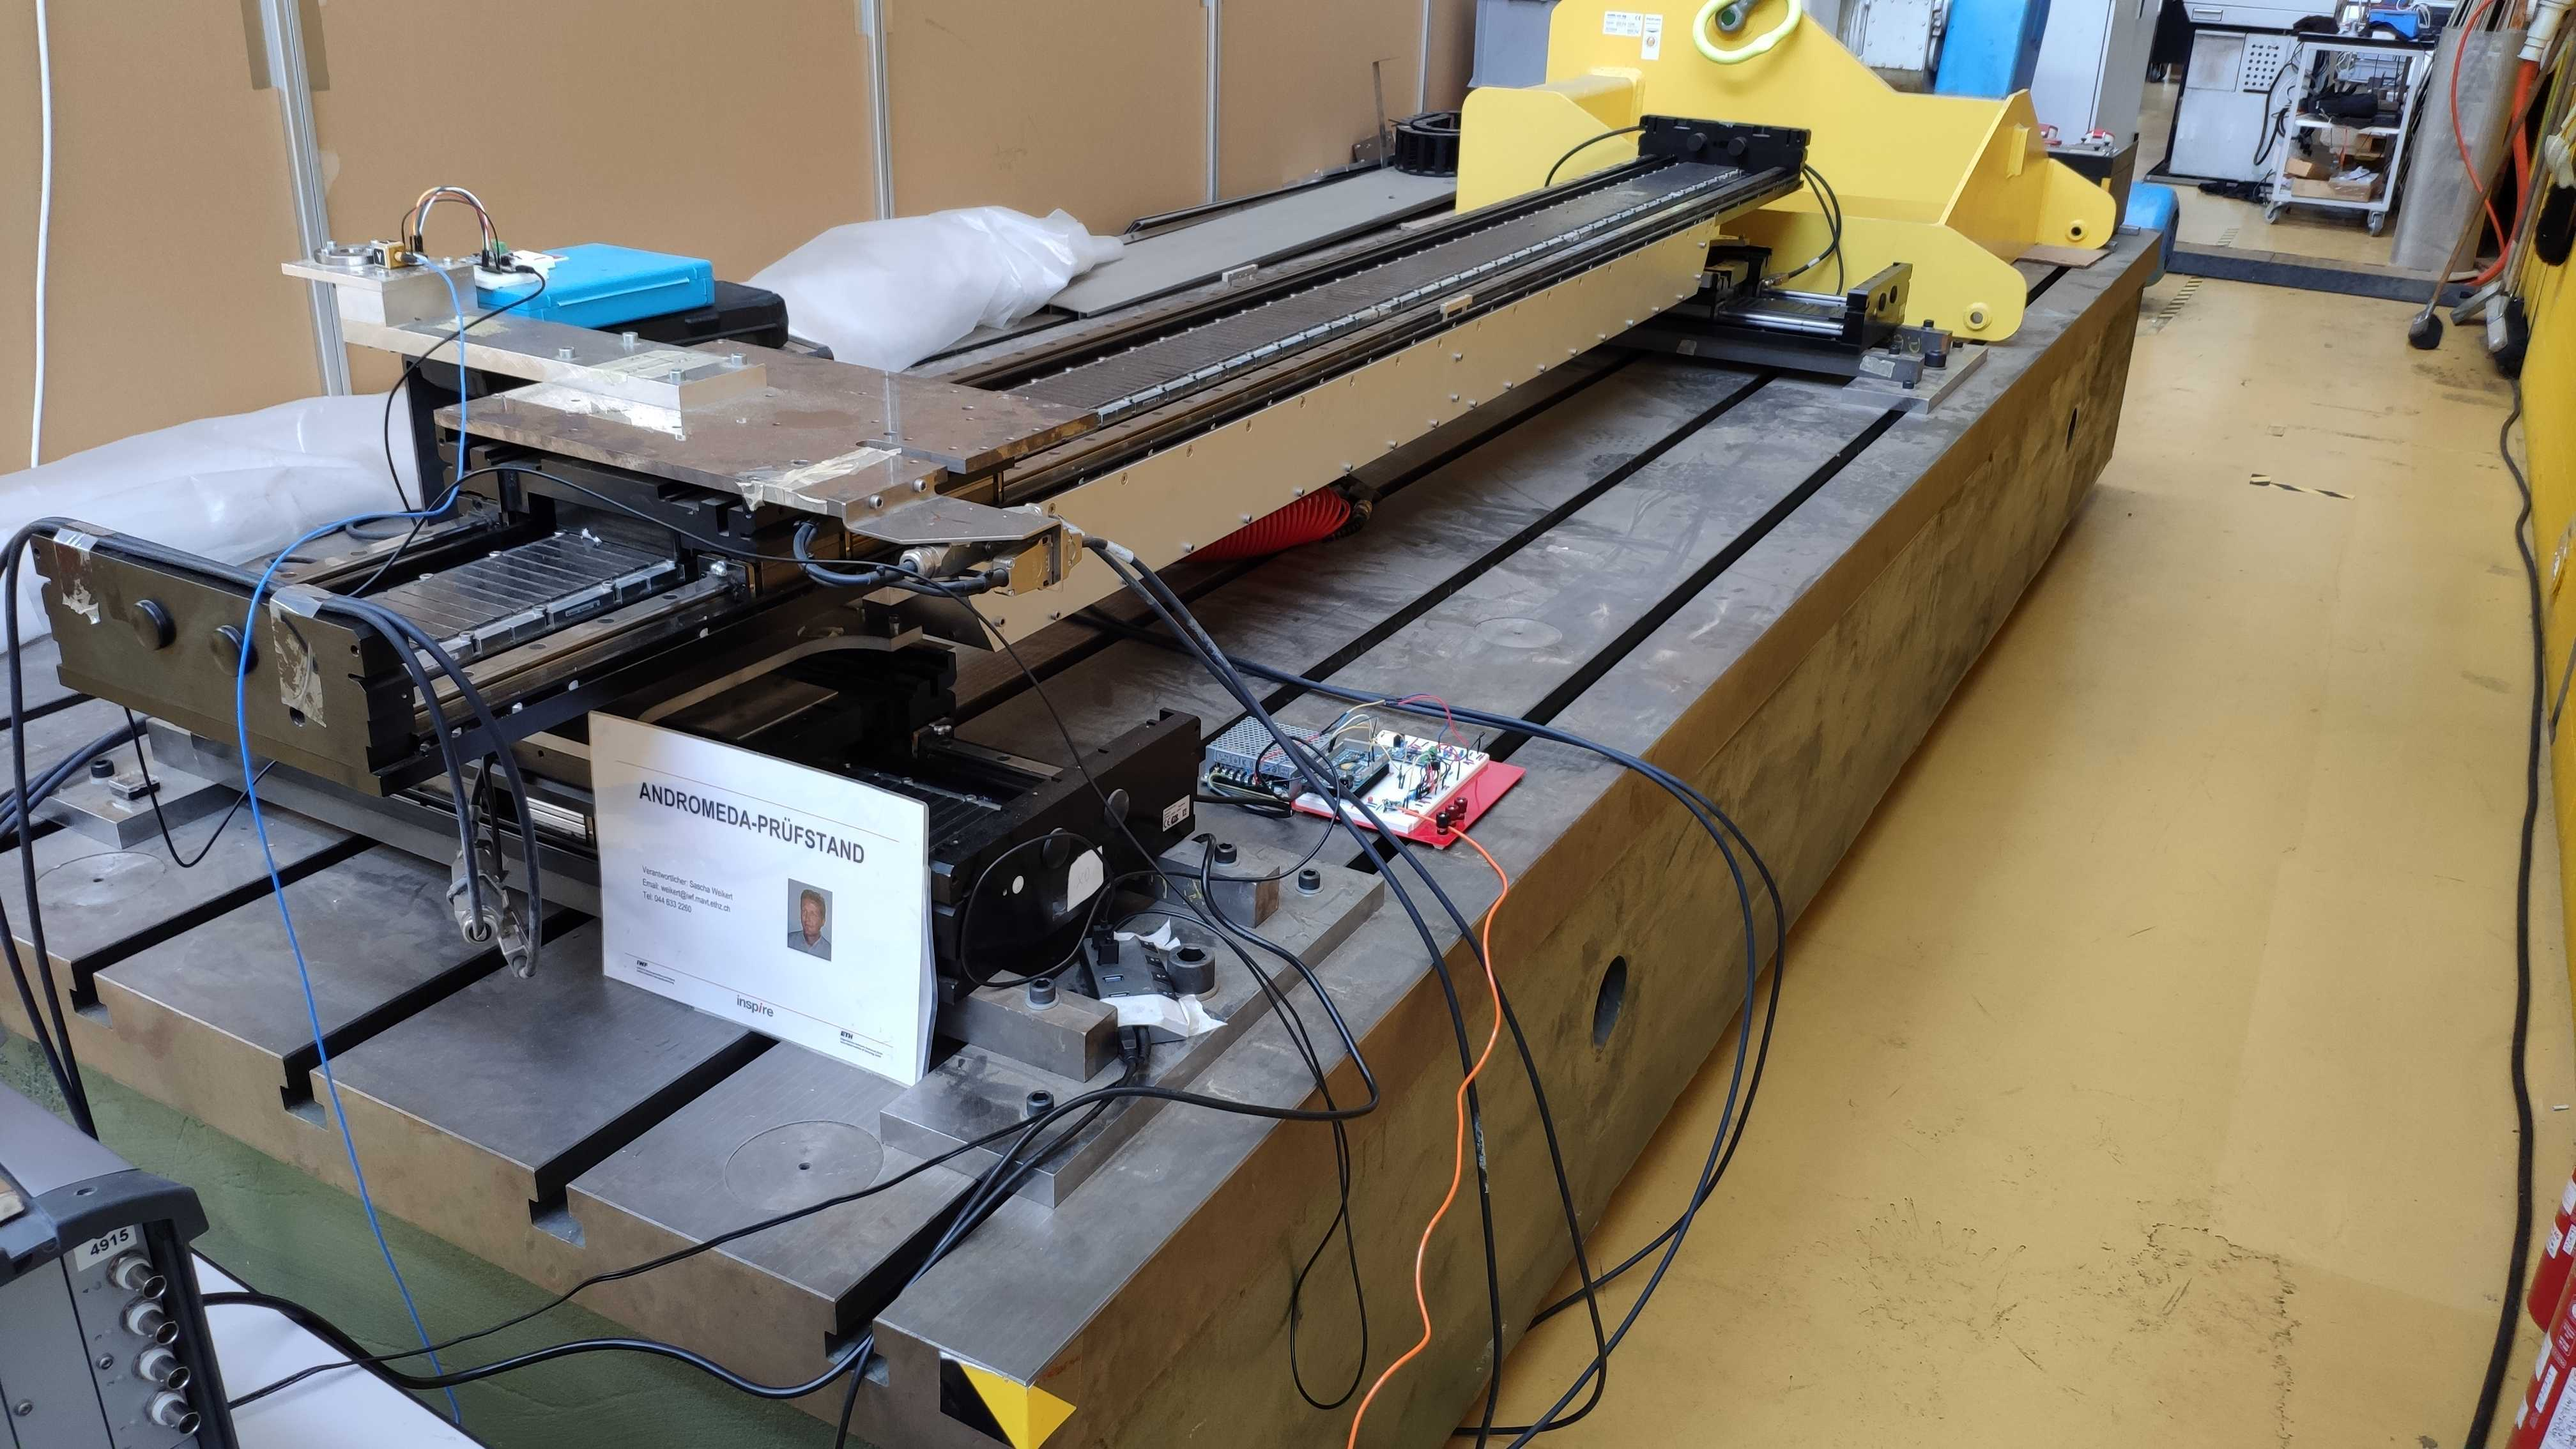
\includegraphics[width=0.50\linewidth]{figures/test_setups/Andromeda/Andromeda_total.jpg}}
    \hspace{4em}
  \subcaptionbox{Acceleromer view\label{sfig:Andromeda_sensors}}{%
    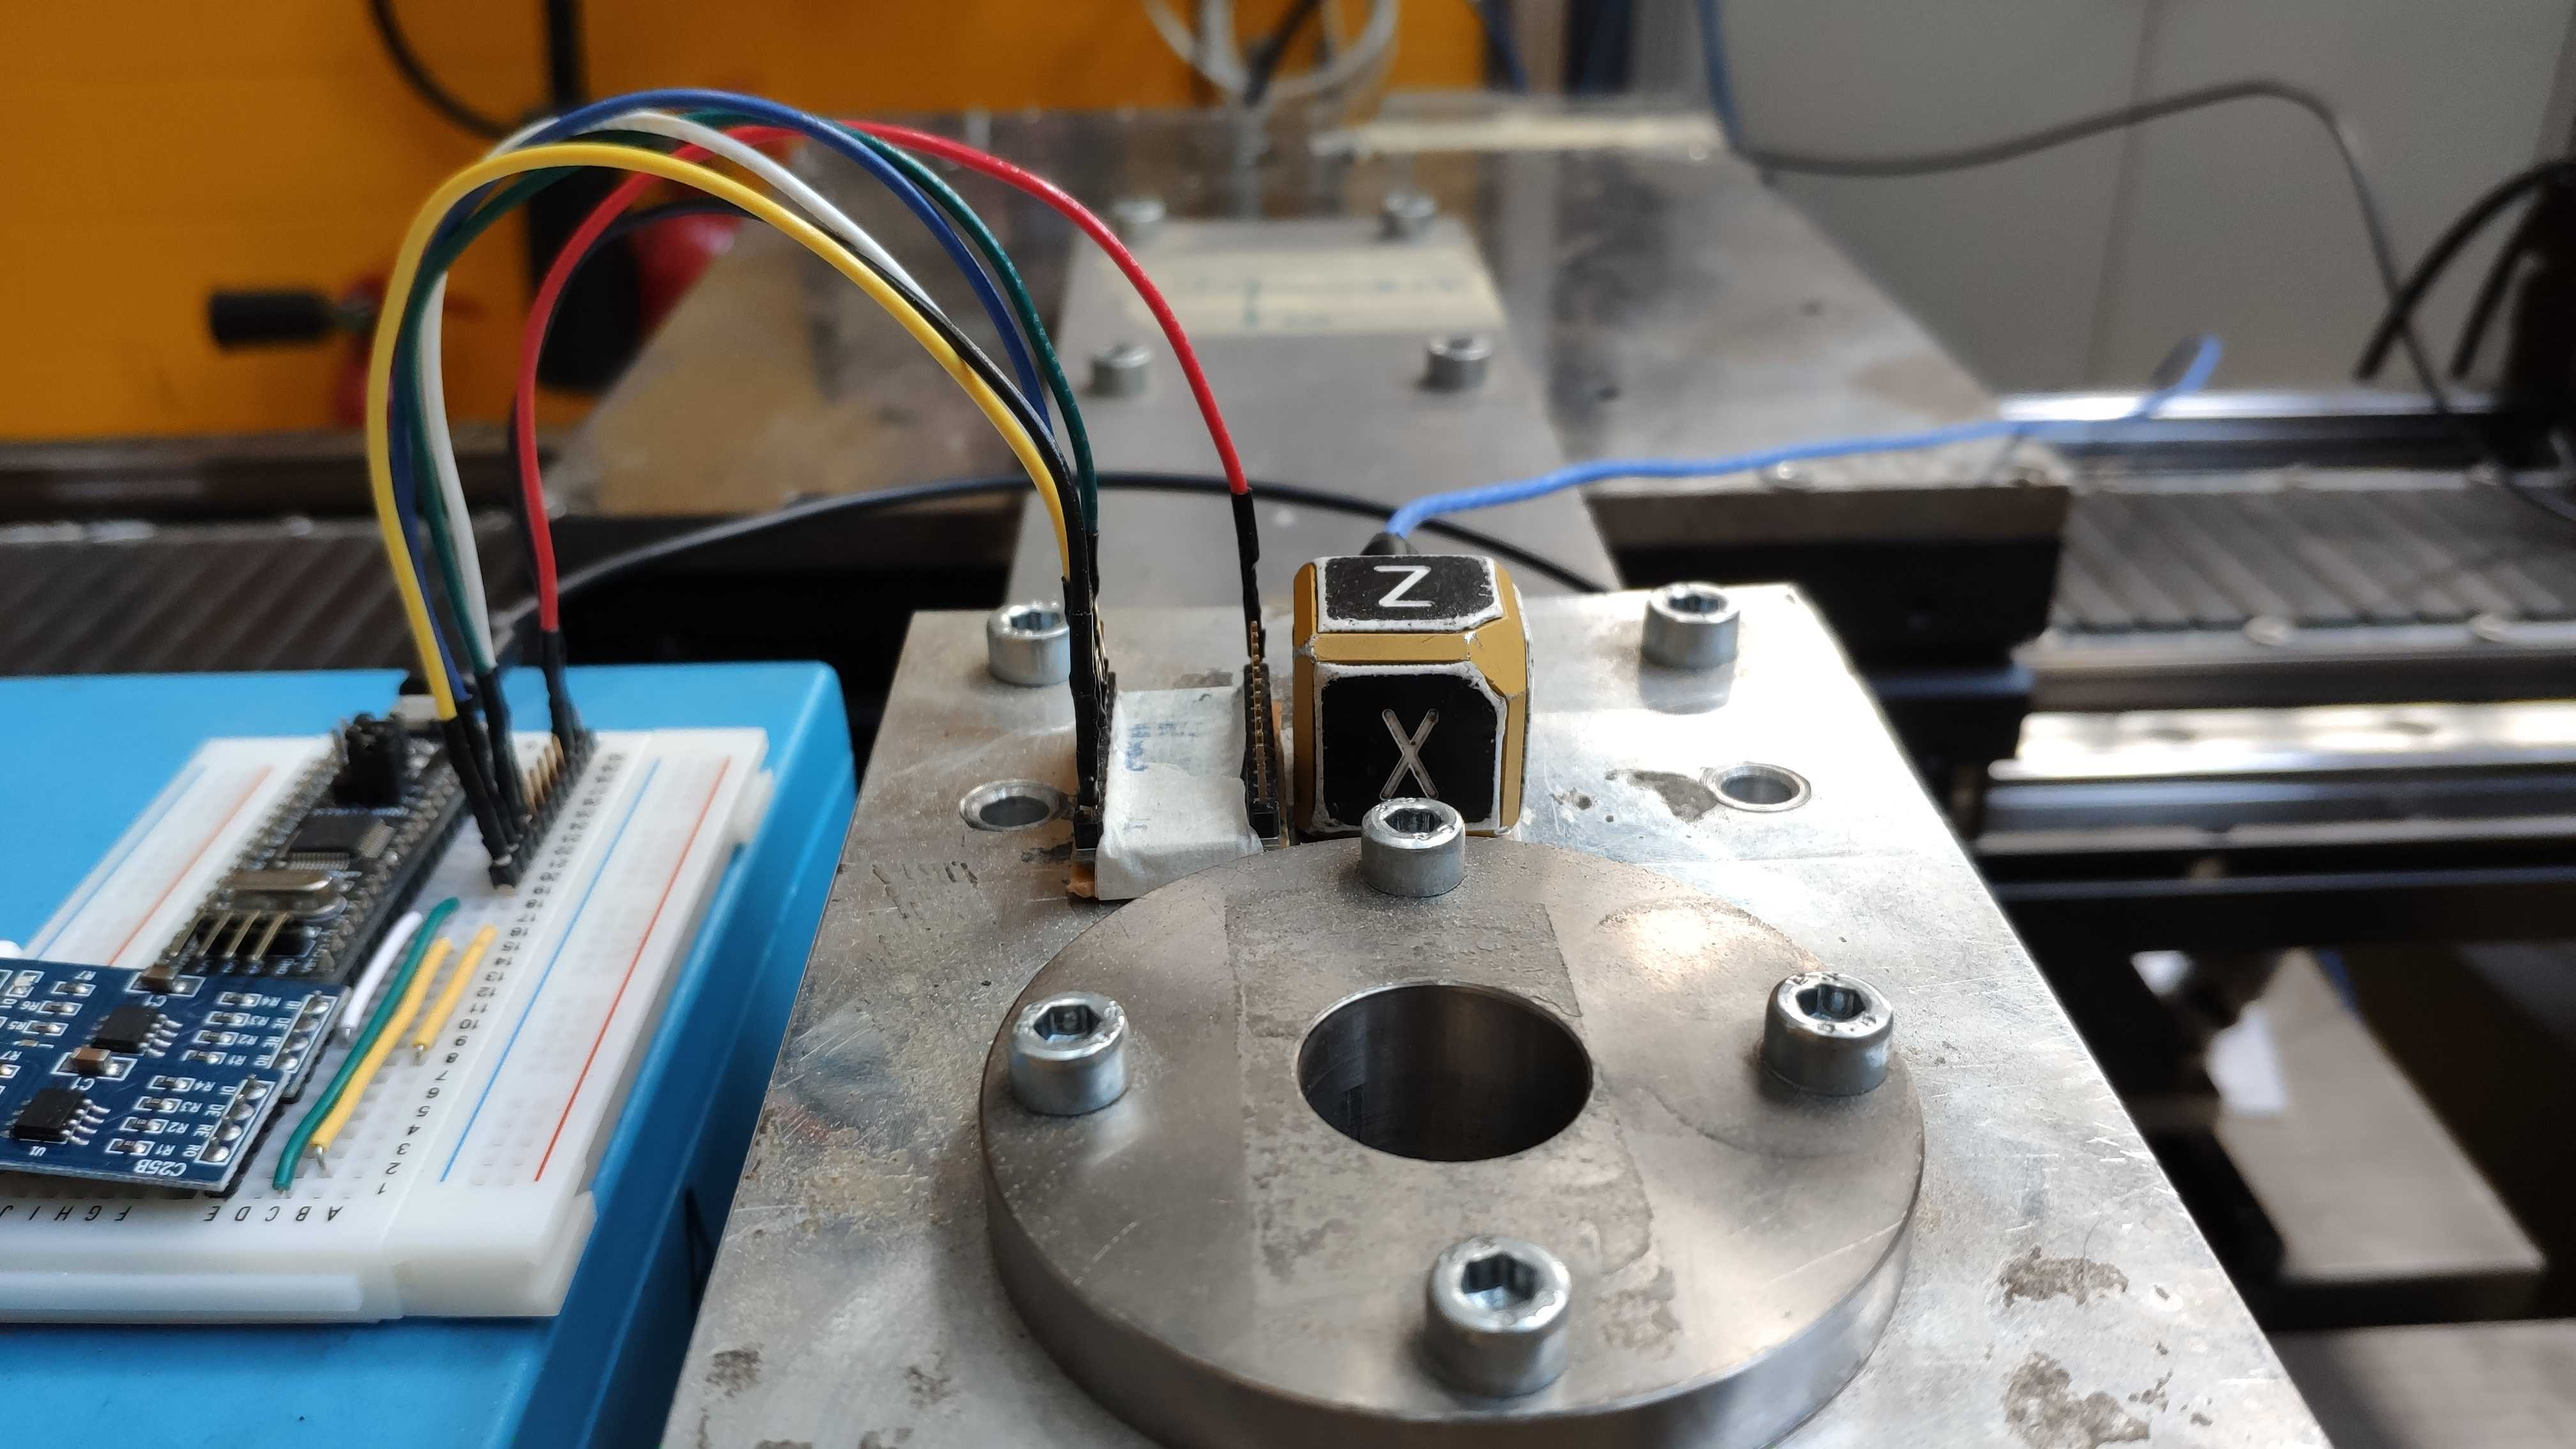
\includegraphics[width=0.3\linewidth]{figures/test_setups/Andromeda/Andromeda_Sensors.jpg}}
  \caption[Andromeda Test Setup]{Andromeda test setup%
    \label{fig:andromeda_pics}}
\end{figure}

\begin{figure}[!htb]
  \centering
  \subcaptionbox{Top view\label{sfig:Andromeda_Positions_Top}}{%
    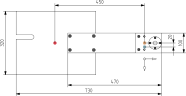
\includegraphics[scale=0.35]{figures/test_setups/Andromeda/Andromeda_Positions_Top}}
    \hspace{4em}
  \subcaptionbox{Trimetric view\label{sfig:Andromeda_Positions_Trimetric_coord}}{%
    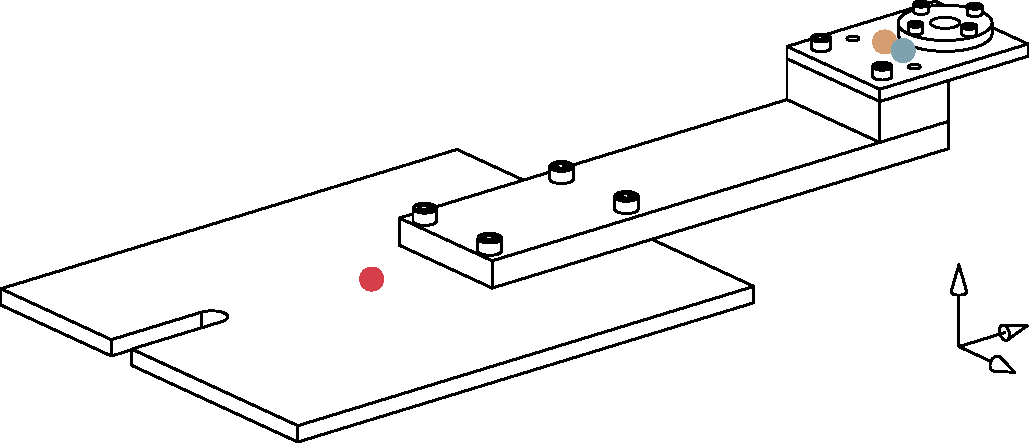
\includegraphics[scale=0.35]{figures/test_setups/Andromeda/Andromeda_Positions_Trimetric_coord}}
  \caption[Andromeda Example Positions]{Andromeda wagon, example impact position%
    \label{fig:andromeda_positions}}
\end{figure}

\section{Filter Test Setups}

The implementation of \ac{DAC} setups as shown in \figref{sfig:dac_comp_precond} required the testing of different filters. For this an Arduino script that allowed the analog-to-digital pins to output a differential sinusoidal signal. The filters then used the differential signal as input and the output was recorded onto the Arduino ADC for signal comparison. Different frequency inputs should verify the filters operation. Namely clock tunable filters, i.e.\ configurable cutoff frequency filters depending on the input frequency of a supply clock have been tested in this setup. For this a variable clock generator module has been used.
